\documentclass[11pt,a4paper]{article}
\usepackage[T1]{fontenc}
\usepackage[utf8]{inputenc}
\usepackage{mathptmx}
\usepackage[a4paper,margin=2.5cm]{geometry}
\usepackage{amsmath,amsthm}
\usepackage{graphicx}
\usepackage{booktabs}
\usepackage{enumitem}
\usepackage[section]{placeins}
\usepackage[font=small,labelfont=bf,labelsep=period]{caption}
\usepackage[hidelinks]{hyperref}
\graphicspath{{figures/}}
\setlength{\parskip}{3pt}
\setlength{\emergencystretch}{1.5em}
\setcounter{secnumdepth}{2}
\renewcommand{\topfraction}{0.9}
\renewcommand{\bottomfraction}{0.8}
\renewcommand{\textfraction}{0.07}
\renewcommand{\floatpagefraction}{0.75}
\renewcommand{\thesection}{\arabic{section}.}
\renewcommand{\thesubsection}{\arabic{section}.\arabic{subsection}.}

\newtheorem{theorem}{Theorem}
\newtheorem{proposition}{Proposition}
\newtheorem{assumption}{Assumption}
\newtheorem{remark}{Remark}
\newcommand{\bv}[1]{\mathbf{#1}}
\newcommand{\Jm}{\boldsymbol{\mathcal{J}}}

\begin{document}

\begin{center}
{\LARGE\bfseries Hybrid Flatness- and Passivity-Based Control with Adaptive RBF Compensation for a 2~MW Direct-Drive PMSG Wind Energy Conversion System\par}
\vspace{12pt}
{\large Said Regani, Manal Messadi and Karim Kemih\,*\par}
\vspace{6pt}
{\small L2EI Laboratory, Jijel University, BP 98, Ouled Aissa, Jijel 18000, Algeria;\\
said.regani@univ-jijel.dz (S.R.); manal.messadi@univ-jijel.dz (M.M.)\\
* Correspondence: karim\_kemih@univ-jijel.dz\par}
\end{center}

\vspace{6pt}
\noindent\textbf{Abstract:} This paper proposes a hybrid nonlinear control scheme for a 2~MW direct-drive
wind energy conversion system based on a permanent magnet synchronous generator (PMSG) connected to the
grid through a back-to-back converter. The scheme combines three layers with distinct roles.
Flatness-based control (FBC) generates the references of the rotor speed and of the energy stored in the
DC link and in the filter, so that the torque and grid-current references are computed directly from the
model. Passivity-based control (PBC) regulates the currents of both converters by energy shaping and
damping injection while keeping the workless coupling terms of the machine and of the filter. An adaptive
radial basis function (RBF) neural network estimates online the lumped aerodynamic-torque and parameter
uncertainty and compensates it in the flat speed law without retuning the nominal gains. A composite
Lyapunov analysis shows that all closed-loop signals remain bounded, that the current errors converge to
zero, and that the speed error converges to a neighborhood of zero whose size depends on the
approximation error of the network. The scheme is evaluated with realistic measurements (sensor noise
and grid voltage harmonics) under step wind, random wind, parameter uncertainty and a 50\,\% grid
voltage dip. All controlled variables track their references, the DC-link voltage remains within
0.8\,\% of its reference outside the dip, the grid-current distortion stays below 4\,\%, and the neural
compensation reduces the integral absolute speed error by 26.5 to 44.8\,\% with the same captured energy.

\vspace{4pt}
\noindent\textbf{Keywords:} wind energy conversion systems; direct-drive PMSG; differential flatness;
passivity-based control; adaptive RBF neural network; Lyapunov stability

%=====================================================================
\section{Introduction}
Wind energy has become one of the main sources of the transition towards low-carbon electricity
generation~\cite{barthelmie2021,iea2024,gwec2024}. Among the variable-speed technologies, the
permanent magnet synchronous generator (PMSG) based wind energy conversion system (WECS) is a preferred
structure for multi-megawatt turbines: in the direct-drive configuration it removes the gearbox, which
improves the efficiency and the reliability~\cite{polinder2013,yaramasu2015}, and its full-scale
back-to-back converter decouples the generator from the grid~\cite{wu2011}. This structure is, however, a
multivariable nonlinear system. The aerodynamic torque depends nonlinearly on the wind speed and on the
rotor speed, the electrical dynamics contain speed-dependent couplings, and the system is subject to
wind variations, torque disturbances, parameter uncertainty and grid disturbances~\cite{rolan2009,aimene2022}.

The machine-side converter (MSC) and the grid-side converter (GSC) are usually controlled by cascaded
proportional-integral (PI) loops in rotating frames, i.e., field-oriented control
(FOC)~\cite{chinchilla2006,yazdani2010,blaabjerg2006}. These controllers are simple to implement, but
they are tuned on a linearized model, so their performance degrades with the nonlinearity and with the
variation of the parameters. Nonlinear alternatives have therefore been proposed to improve the tracking,
the power quality and the robustness. Sliding mode control (SMC) was applied to wind turbines with an
exponential reaching law~\cite{mechter2015} and, for a chaotic PMSG in an offshore turbine, in a
chattering-free terminal form~\cite{benabdeeseelam2025}. Backstepping was used at low wind
speeds~\cite{mechter2016}, predictive control was applied to a chaotic PMSG~\cite{messadi2015}, and a
fuzzy state-feedback control was designed for a fractional-order direct-drive PMSG with uncertain
parameters~\cite{yang2021}.

Two model-based methods are particularly suited to the structure of the WECS. Differential
flatness~\cite{fliess1995} expresses all the variables of a system from a flat output and its
derivatives; it therefore generates the references of the inner variables directly from the desired
trajectory, which is valuable during transients and sudden wind changes. Aimene et al.~\cite{aimene2022}
showed that flatness-based control improves the transients of a grid-connected PMSG system with respect
to FOC, and Thounthong et al.~\cite{thounthong2010} showed that, with the stored energy as flat output,
the DC-bus dynamics become a linear power balance. Passivity-based control (PBC)~\cite{ortega1998,ortega2002}
shapes the energy of the closed loop and injects damping while keeping the physical, workless couplings
instead of cancelling them, which gives a robust current control with a clear energy interpretation.
Both methods use a model, and their weak point is the aerodynamic torque, which is not measured, and the
parameters of the generator.

Learning-based approximators can address this weak point. RBF networks are universal
approximators~\cite{park1991} whose weights can be adapted online by a Lyapunov-based
law~\cite{lewis1999,ioannou1996}. They were combined with terminal sliding mode control~\cite{li2024}, with
observer-based adaptive control~\cite{bounar2025} and with data-driven tuning under real wind
profiles~\cite{dardabi2024}. In our previous work~\cite{regani2026}, an adaptive neural network
compensated the residual tracking error of a nonlinear state-feedback controller without retuning its
gains, but measurement noise and grid disturbances were not considered. To the authors' knowledge, a
scheme in which flatness generates the references, PBC guarantees the energy structure and the damping of
the current loops of both converters, and an adaptive RBF network compensates the uncertainty, evaluated
under realistic measurements and grid disturbances, has not been reported for a multi-megawatt
direct-drive PMSG.

The main contributions of this work are as follows:
\begin{itemize}[leftmargin=*,itemsep=2pt]
\item \textbf{Flatness-based reference generation:} the rotor speed and the energy of the DC link and of
the filter are used as flat outputs; the torque and grid-current references are computed directly from
the model, and the DC-link dynamics become a linear power balance.
\item \textbf{Passivity-based inner control:} the currents of both converters are controlled by energy
shaping and damping injection, with a storage function that proves the convergence of the current errors.
\item \textbf{Adaptive RBF compensation:} an RBF network estimates online the lumped aerodynamic-torque and
parameter uncertainty and compensates it in the flat speed law, with the nominal gains unchanged.
\item \textbf{Composite Lyapunov stability analysis:} the boundedness of all closed-loop signals and the
convergence of the tracking errors to a neighborhood of zero are proved.
\item \textbf{Realistic numerical validation:} the scheme is evaluated with sensor noise and grid harmonics
under step wind, random wind, parameter uncertainty and a grid voltage dip, without and with the neural
compensation.
\end{itemize}

The paper is organized as follows. Section~2 describes and models the system. Section~3 states the
control objectives and the MPPT strategy. Sections~4, 5 and 6 present the flatness-based reference
generation, the passivity-based inner control and the adaptive RBF compensation. Section~7 analyzes the
stability. Section~8 presents and discusses the simulation results, and Section~9 concludes the paper.

%=====================================================================
\section{System Description and Modeling}
\subsection{System Configuration}
The overall configuration of the studied system is shown in Figure~\ref{fig:system}. The wind turbine
drives the PMSG directly, without gearbox. The MSC rectifies the generator voltages and controls the
generator currents, the DC link decouples the two converters, and the GSC injects the power into the
690~V, 50~Hz grid through an $L$ filter. The parameters are given in Table~\ref{tab:param}.

\begin{figure}[!htb]
\centering
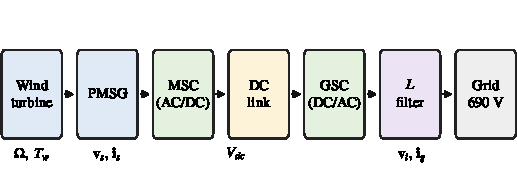
\includegraphics[width=0.75\textwidth]{system.pdf}
\caption{Overall configuration of the 2~MW direct-drive PMSG wind energy conversion system.}
\label{fig:system}
\end{figure}

\subsection{Wind Turbine Aerodynamics}
The tip-speed ratio, the mechanical power and the aerodynamic torque are~\cite{heier2014,aimene2022}
\begin{equation}
\lambda=\frac{\Omega R}{v},\qquad P_w=\tfrac{1}{2}\rho\pi R^2 C_p(\lambda,\beta)\,v^3,\qquad T_w=\frac{P_w}{\Omega},
\label{eq:pw}
\end{equation}
where $\rho$ is the air density, $R$ the rotor radius, $v$ the wind speed, $\Omega$ the rotor speed and
$\beta$ the pitch angle. The power coefficient is
\begin{equation}
C_p = 0.5176\Bigl(\frac{116}{\lambda_i}-0.4\beta-5\Bigr)e^{-21/\lambda_i}+0.0068\lambda,\qquad
\frac{1}{\lambda_i}=\frac{1}{\lambda+0.08\beta}-\frac{0.035}{\beta^3+1}.
\label{eq:cp}
\end{equation}
For $\beta=0$, $C_p$ reaches $C_{p,\max}=0.48$ at $\lambda^\star=8.1$. For $P_n=2$~MW and $R=40$~m, the
rated wind speed given by $P_n=\frac12\rho\pi R^2C_{p,\max}v_n^3$ is $v_n=11.0$~m/s, the rated speed is
$\Omega_n=\lambda^\star v_n/R=2.23$~rad/s and the rated torque is $T_n=P_n/\Omega_n=0.897$~MN$\cdot$m.
Since the wind remains below $v_n$ in this study, the pitch angle is kept at zero.

\subsection{PMSG Model in the $dq$ Frame}
In the rotor $dq$ frame (amplitude-invariant transformation, $d$ axis aligned with the magnet flux),
with the receptor convention and $L_d=L_q=L_s$~\cite{aimene2022},
\begin{align}
v_{sd} &= R_s i_{sd} + L_s\frac{di_{sd}}{dt} - \omega_e L_s i_{sq},\label{eq:vsd}\\
v_{sq} &= R_s i_{sq} + L_s\frac{di_{sq}}{dt} + \omega_e L_s i_{sd} + \omega_e\psi_f,\label{eq:vsq}\\
T_e &= \tfrac32 p\,\psi_f\, i_{sq},\label{eq:te}
\end{align}
where $\omega_e=p\Omega$, $p$ is the number of pole pairs and $\psi_f$ the magnet flux; $T_e<0$ and
$i_{sq}<0$ in generating mode. With $\bv{i}_s=[i_{sd}\;i_{sq}]^T$, $\bv{v}_s=[v_{sd}\;v_{sq}]^T$,
$\bv{e}_q=[0\;1]^T$ and the skew-symmetric matrix
$\Jm=\bigl[\begin{smallmatrix}0&1\\-1&0\end{smallmatrix}\bigr]$,
\begin{equation}
L_s\dot{\bv{i}}_s = \bv{v}_s - R_s\bv{i}_s + \omega_eL_s\Jm\bv{i}_s - \omega_e\psi_f\bv{e}_q .
\label{eq:pmsg}
\end{equation}
The generator data are those of the non-salient 2~MW PMSG of~\cite{hasan2021}.

\subsection{Drive Train}
The direct-drive shaft is described by the one-mass model
\begin{equation}
J\frac{d\Omega}{dt} = T_w + T_e - B\Omega ,
\label{eq:shaft}
\end{equation}
where $J$ is the total inertia and $B$ the friction coefficient.

\subsection{DC Link and Grid Side}
The converters are represented by their average model, with voltage vectors limited to $V_{dc}/\sqrt3$.
The DC-link voltage obeys~\cite{aimene2022}
\begin{equation}
CV_{dc}\frac{dV_{dc}}{dt} = P_{dc} - P_i,\qquad P_{dc}=-\tfrac32\bv{v}_s^T\bv{i}_s,\qquad
P_i=\tfrac32\bv{v}_i^T\bv{i}_g ,
\label{eq:dc}
\end{equation}
where $\bv{v}_i$ is the GSC voltage and $\bv{i}_g$ the grid current. In the grid-voltage-oriented frame
($v_{gq}=0$), with the current counted towards the grid,
\begin{equation}
L_f\dot{\bv{i}}_g = \bv{v}_i - R_f\bv{i}_g + \omega_gL_f\Jm\bv{i}_g - \bv{v}_g ,
\label{eq:filter}
\end{equation}
and the grid powers are $P_g=\frac32v_{gd}i_{gd}$ and $Q_g=-\frac32v_{gd}i_{gq}$.

\subsection{Energy Balance}
With $E=\frac12J\Omega^2+\frac34L_s\|\bv{i}_s\|^2+\frac12CV_{dc}^2+\frac34L_f\|\bv{i}_g\|^2$, and since
$\bv{x}^T\Jm\bv{x}=0$ and $T_e\Omega=\frac32\omega_e\psi_fi_{sq}$, the model (\ref{eq:pw})--(\ref{eq:filter})
gives, for any state and any converter voltages,
\begin{equation}
\dot E = P_w - B\Omega^2 - \tfrac32R_s\|\bv{i}_s\|^2 - \tfrac32R_f\|\bv{i}_g\|^2 - P_g .
\label{eq:balance}
\end{equation}
This balance verifies the sign of every term of the model; its numerical residual is below
$10^{-15}P_n$. It also shows the energy structure used by the PBC design of Section~5.

\begin{table}[!htb]
\caption{Parameters of the studied system and of the simulation.}
\label{tab:param}
\centering
\setlength{\tabcolsep}{5pt}
\begin{tabular}{llll}
\toprule
Group & Parameter & Value & Source\\
\midrule
Turbine & rotor radius $R$, air density $\rho$ & 40 m, 1.225 kg/m$^3$ & \cite{rolan2009,aimene2022}\\
 & pitch angle $\beta$, $C_p$ model & 0, (\ref{eq:cp}) & \cite{heier2014}\\
 & $C_{p,\max}$, $\lambda^\star$, $v_n$, $\Omega_n$ & 0.48, 8.1, 11.0 m/s, 2.23 rad/s & (\ref{eq:pw})\\
PMSG & rated power $P_n$, pole pairs $p$ & 2 MW, 26 & \cite{hasan2021}\\
 & $R_s$, $L_d=L_q=L_s$, $\psi_f$ & 0.78 m$\Omega$, 1.57 mH, 9.18 Wb & \cite{hasan2021}\\
 & inertia $J$, friction $B$ & $2.8\times10^6$ kg$\cdot$m$^2$, $10^3$ N$\cdot$m$\cdot$s & assumed\\
DC link and grid & $C$, $V_{dc}^*$ & 20 mF, 1200 V & \cite{hasan2021}\\
 & $L_f$, $R_f$ & 0.15 mH, 2 m$\Omega$ & \cite{hasan2021}, assumed\\
 & $V_g$ (line-to-line rms), $\omega_g$ & 690 V, $2\pi\cdot50$ rad/s & \cite{hasan2021}\\
Simulation setup & switching frequency $f_{sw}$ & 2160 Hz & \cite{hasan2021}\\
 & sampling time $T_s=1/(2f_{sw})$ & 231.5 $\mu$s & \\
 & solver & fixed-step Runge--Kutta 4, step $T_s$ & \\
\bottomrule
\end{tabular}
\end{table}

%=====================================================================
\section{Control Objectives and MPPT Strategy}
\subsection{Control Objectives}
The control is shared between the two converters:
\begin{itemize}[leftmargin=*,itemsep=2pt]
\item the MSC tracks the optimal rotor speed, in order to extract the maximum power below the rated
wind speed, and keeps $i_{sd}=0$, which minimizes the copper losses of the non-salient machine;
\item the GSC regulates the DC-link voltage at $V_{dc}^*=1200$~V, injects the active power into the grid
and keeps the reactive power at zero, i.e., a unity power factor ($i_{gq}=0$).
\end{itemize}
All the errors are defined as measured minus reference values. The controller is sampled at $T_s$, and
the converter voltages are applied one sample after their computation.

\subsection{Tip-Speed-Ratio MPPT}
The tip-speed-ratio (TSR) MPPT is used. The optimal speed
\begin{equation}
\Omega_{opt}=\frac{\lambda^\star v_m}{R},
\label{eq:mppt}
\end{equation}
computed from the anemometer measurement $v_m$ and limited to $[0.5\Omega_n,\Omega_n]$, is filtered by
the second-order model
\begin{equation}
\ddot\Omega^*=\omega_r^2(\Omega_{opt}-\Omega^*)-2\omega_r\dot\Omega^* ,
\label{eq:ref}
\end{equation}
with $\omega_r=1$~rad/s. This filter gives a smooth reference $\Omega^*$ and its derivative
$\dot\Omega^*$, which are required by the flatness-based law of Section~4, and it avoids demanding fast
speed changes that the large inertia of the turbine cannot follow.

%=====================================================================
\section{Flatness-Based Reference Generation}
A system is differentially flat when all its variables can be expressed as functions of a flat output
and of a finite number of its derivatives~\cite{fliess1995}. This property is used here to generate the
references of the inner variables directly from the desired trajectories, instead of using cascaded
loops that react only after an error has appeared~\cite{aimene2022}. The resulting reference generator is
shown in Figure~\ref{fig:fbc}, and the flat outputs are summarized in Table~\ref{tab:flat}.

\begin{figure}[!htb]
\centering
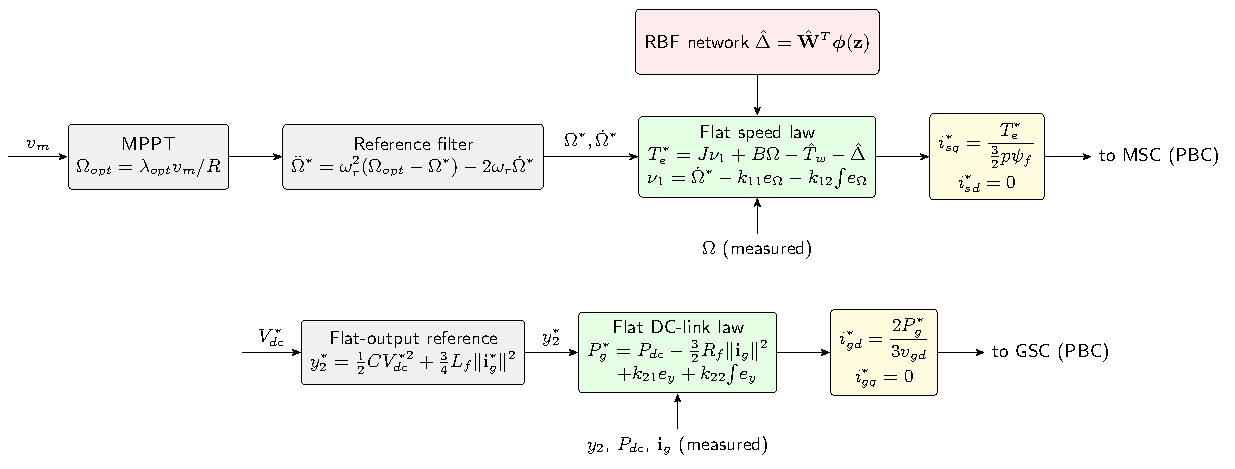
\includegraphics[width=\textwidth]{fbc.pdf}
\caption{Flatness-based reference generation for the MSC (top) and for the GSC (bottom).}
\label{fig:fbc}
\end{figure}

\subsection{Speed Loop}
For the PMSG and the shaft, $(\Omega, i_{sd})$ is a flat output: from (\ref{eq:shaft}) and (\ref{eq:te}),
\begin{equation}
T_e=J\dot\Omega+B\Omega-T_w,\qquad i_{sq}=\frac{T_e}{\frac32p\psi_f},
\end{equation}
and the voltages follow from (\ref{eq:vsd})--(\ref{eq:vsq}) with $i_{sd}$, $i_{sq}$ and their
derivatives. Imposing $\dot\Omega=\nu_1$ with
\begin{equation}
\nu_1=\dot\Omega^*-k_{11}e_\Omega-k_{12}\!\int\!e_\Omega\,dt,\qquad e_\Omega=\Omega-\Omega^*,
\end{equation}
gives the torque and current references
\begin{equation}
T_e^* = J\nu_1 + B\Omega - \hat T_w - \hat\Delta,\qquad i_{sq}^*=\frac{T_e^*}{\frac32p\psi_f},\qquad i_{sd}^*=0,
\label{eq:flat1}
\end{equation}
where $\hat T_w$ is computed from (\ref{eq:pw})--(\ref{eq:cp}) with $v_m$, and $\hat\Delta$ is the neural
compensation of Section~6 ($\hat\Delta=0$ for the nominal controller). $T_e^*$ is limited to
$[-1.2T_n,0]$, with the integration frozen at the limit.

\subsection{DC-Link Loop}
For the GSC, the flat output is the energy stored in the DC link and in the filter,
$y_2=\frac12CV_{dc}^2+\frac34L_f\|\bv{i}_g\|^2$, together with $i_{gq}$. From (\ref{eq:dc})--(\ref{eq:filter}),
\begin{equation}
\dot y_2 = P_{dc} - P_g - \tfrac32R_f\|\bv{i}_g\|^2 ,
\label{eq:y2}
\end{equation}
which is a linear power balance~\cite{thounthong2010}. Imposing $\dot y_2=-k_{21}e_y-k_{22}\int e_y\,dt$,
with $e_y=y_2-y_2^*$ and $y_2^*=\frac12CV_{dc}^{*2}+\frac34L_f\|\bv{i}_g^*\|^2$, gives
\begin{equation}
P_g^* = P_{dc} - \tfrac32R_f\|\bv{i}_g\|^2 + k_{21}e_y + k_{22}\!\int\! e_y\,dt,\qquad
i_{gd}^*=\frac{2P_g^*}{3v_{gd}},\qquad i_{gq}^*=0 .
\label{eq:flat2}
\end{equation}
The feedforward of $P_{dc}$, computed from the applied MSC voltages and the measured currents, passes the
generator power to the grid before it changes $V_{dc}$.

\begin{table}[!htb]
\caption{Flat outputs, reference variables and required derivatives.}
\label{tab:flat}
\centering
\begin{tabular}{llll}
\toprule
Subsystem & Flat output & References generated & Required derivatives\\
\midrule
PMSG and shaft (MSC) & $\Omega$, $i_{sd}$ & $T_e^*$, $i_{sq}^*$ (\ref{eq:flat1}); $i_{sd}^*=0$ & $\dot\Omega^*$ from (\ref{eq:ref}); $\dot{\bv{i}}_s^*$\\
DC link and filter (GSC) & $y_2$, $i_{gq}$ & $P_g^*$, $i_{gd}^*$ (\ref{eq:flat2}); $i_{gq}^*=0$ & $\dot y_2$ from (\ref{eq:y2}); $\dot{\bv{i}}_g^*$\\
Current loops (PBC) & -- & $\bv{v}_s^*$, $\bv{v}_i^*$ (Section 5) & first-order filters (2 ms)\\
\bottomrule
\end{tabular}
\end{table}

%=====================================================================
\section{Passivity-Based Inner Control Design}
\subsection{Port-Controlled Hamiltonian Form}
With the stored magnetic energy $H_s=\frac12L_s\|\bv{i}_s\|^2$, the generator model (\ref{eq:pmsg}) is a
port-controlled Hamiltonian system with dissipation~\cite{ortega2002}:
\begin{equation}
L_s\dot{\bv{i}}_s = \bigl(\omega_eL_s\Jm - R_s\bv{I}\bigr)\bv{i}_s + \bv{v}_s - \omega_e\psi_f\bv{e}_q ,
\qquad \dot H_s = -R_s\|\bv{i}_s\|^2 + \bv{i}_s^T(\bv{v}_s-\omega_e\psi_f\bv{e}_q) .
\label{eq:pch}
\end{equation}
The interconnection term $\omega_eL_s\Jm$ is skew-symmetric, so it does not produce or dissipate energy.
PBC keeps this workless term instead of cancelling it, shapes the energy of the error dynamics, and
injects damping~\cite{ortega1998}. The structure is shown in Figure~\ref{fig:pbc}.

\begin{figure}[!htb]
\centering
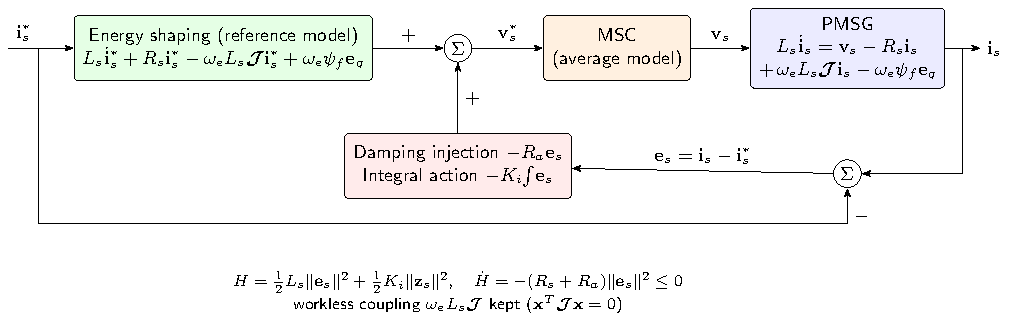
\includegraphics[width=0.95\textwidth]{pbc.pdf}
\caption{Energy-shaping and damping-injection structure of the passivity-based current control (MSC).}
\label{fig:pbc}
\end{figure}

\subsection{Machine-Side Control Law}
With $\bv{e}_s=\bv{i}_s-\bv{i}_s^*$ and $\dot{\bv{z}}_s=\bv{e}_s$, the MSC voltage reference is
\begin{equation}
\bv{v}_s^* = \underbrace{L_s\dot{\bv{i}}_s^* + R_s\bv{i}_s^* - \omega_eL_s\Jm\bv{i}_s^* + \omega_e\psi_f\bv{e}_q}_{\text{energy shaping}}
\underbrace{- R_a\bv{e}_s}_{\text{damping}} - K_i\bv{z}_s .
\label{eq:pbc1}
\end{equation}
Inserting (\ref{eq:pbc1}) into (\ref{eq:pmsg}) gives the error dynamics
\begin{equation}
L_s\dot{\bv{e}}_s=-(R_s+R_a)\bv{e}_s+\omega_eL_s\Jm\bv{e}_s-K_i\bv{z}_s ,
\label{eq:es}
\end{equation}
which keep the skew-symmetric coupling of the machine, with the total damping $R_s+R_a$.

\subsection{Grid-Side Control Law}
The same design is applied to the filter (\ref{eq:filter}). With $\bv{e}_g=\bv{i}_g-\bv{i}_g^*$ and
$\dot{\bv{z}}_g=\bv{e}_g$,
\begin{equation}
\bv{v}_i^* = L_f\dot{\bv{i}}_g^* + R_f\bv{i}_g^* - \omega_gL_f\Jm\bv{i}_g^* + \bv{v}_g
- R_b\bv{e}_g - K_{ig}\bv{z}_g ,
\label{eq:pbc2}
\end{equation}
which gives $L_f\dot{\bv{e}}_g=-(R_f+R_b)\bv{e}_g+\omega_gL_f\Jm\bv{e}_g-K_{ig}\bv{z}_g$. The reference
derivatives are obtained by first-order filters with a time constant of 2~ms, and the integrals are
frozen when the voltage reaches $V_{dc}/\sqrt3$.

\begin{proposition}
With $R_a,K_i>0$, the storage function $H_e=\frac12L_s\|\bv{e}_s\|^2+\frac12K_i\|\bv{z}_s\|^2$ of the
error dynamics (\ref{eq:es}) satisfies $\dot H_e=-(R_s+R_a)\|\bv{e}_s\|^2\le0$. The same holds for the
grid side with $H_g=\frac12L_f\|\bv{e}_g\|^2+\frac12K_{ig}\|\bv{z}_g\|^2$ and
$\dot H_g=-(R_f+R_b)\|\bv{e}_g\|^2$.
\end{proposition}
\begin{proof}
From (\ref{eq:es}), $\dot H_e=\bv{e}_s^TL_s\dot{\bv{e}}_s+K_i\bv{z}_s^T\bv{e}_s=-(R_s+R_a)\|\bv{e}_s\|^2
+\omega_eL_s\bv{e}_s^T\Jm\bv{e}_s=-(R_s+R_a)\|\bv{e}_s\|^2$, since $\bv{e}_s^T\Jm\bv{e}_s=0$. The grid
side is identical.
\end{proof}

The gains place double closed-loop poles: $R_s+R_a=2\omega_iL_s$, $K_i=\omega_i^2L_s$,
$R_f+R_b=2\omega_iL_f$, $K_{ig}=\omega_i^2L_f$, $k_{11}=2\omega_\Omega$, $k_{12}=\omega_\Omega^2$,
$k_{21}=2\omega_v$ and $k_{22}=\omega_v^2$, with $\omega_i=500$, $\omega_v=60$ and $\omega_\Omega=2$~rad/s,
so that the bandwidths are separated by more than one decade (Table~\ref{tab:rbf}).

%=====================================================================
\section{Adaptive RBF Neural Compensation}
\subsection{Lumped Uncertainty}
The flat speed law (\ref{eq:flat1}) uses the model $\hat T_w$ of the aerodynamic torque. The $C_p$
model, the anemometer, which measures the wind at one point and with a delay, the magnet flux and the
other parameters of the generator are uncertain. Their effects are gathered in the lumped uncertainty
\begin{equation}
\Delta(\bv{x},t)=T_w-\hat T_w ,
\end{equation}
and, with $i_{sq}=i_{sq}^*$, the speed error obeys
\begin{equation}
J\bigl(\dot e_\Omega + k_{11}e_\Omega + k_{12}\!\textstyle\int\! e_\Omega\,dt\bigr) = \Delta-\hat\Delta .
\label{eq:errw}
\end{equation}

\subsection{RBF Approximation}
The uncertainty depends mainly on the operating point, i.e., on the rotor speed and on the wind speed.
The input vector of the network is
\begin{equation}
\bv{z}=\Bigl[\frac{\Omega}{\Omega_n}\;\;\frac{v_m}{v_n}\Bigr]^T ,
\label{eq:z}
\end{equation}
and, on a compact operating region $\Omega_z$, the uncertainty is approximated by~\cite{park1991}
\begin{equation}
\Delta=\bv{W}^{*T}\boldsymbol\Phi(\bv{z})+\varepsilon,\qquad |\varepsilon|\le\bar\varepsilon ,\qquad
\Phi_j(\bv{z})=\exp\Bigl(-\frac{\|\bv{z}-\bv{c}_j\|^2}{2b^2}\Bigr),
\label{eq:approx}
\end{equation}
where $\bv{W}^*$ is an ideal weight vector and $\varepsilon$ the approximation error. The network has 25
Gaussian units centred on a $5\times5$ grid of $[0.5,1.1]^2$ with the width $b=0.15$
(Table~\ref{tab:rbf}). The compensation term is
\begin{equation}
\hat\Delta(\bv{z})=\hat{\bv{W}}^T\boldsymbol\Phi(\bv{z}) .
\label{eq:dh}
\end{equation}
When the network is used, it replaces the integral action of the speed loop ($k_{12}=0$); otherwise the
integral would absorb the slowly varying part of $\Delta$ and the network would not learn it.

\subsection{Adaptation Law}
The weights are adapted online by the Lyapunov-based law with $\sigma$-modification~\cite{ioannou1996}
\begin{equation}
\dot{\hat{\bv{W}}} = \Gamma\bigl(\boldsymbol\Phi(\bv{z})\,e_\Omega - \sigma\hat{\bv{W}}\bigr),\qquad
\hat{\bv{W}}(0)=0,
\label{eq:law}
\end{equation}
where $\Gamma>0$ is the adaptation gain and $\sigma>0$ limits the drift of the weights in the presence of
noise and approximation error. The adaptation is frozen when $T_e^*$ reaches its limit. The complete
controller is shown in Figure~\ref{fig:structure}.

\begin{figure}[!htb]
\centering
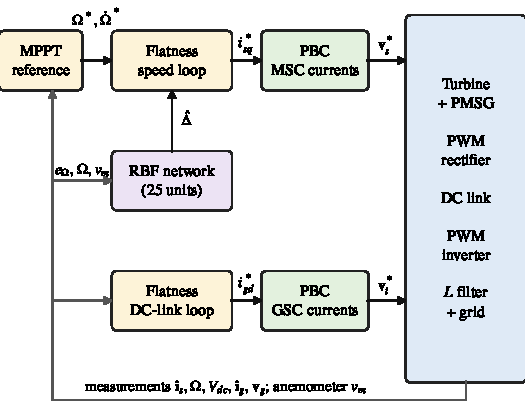
\includegraphics[width=0.7\textwidth]{structure.pdf}
\caption{Complete proposed controller: flatness-based references, passivity-based current loops and
adaptive RBF compensation.}
\label{fig:structure}
\end{figure}

\begin{table}[!htb]
\caption{RBF network and controller parameters.}
\label{tab:rbf}
\centering
\begin{tabular}{ll}
\toprule
Parameter & Value\\
\midrule
RBF inputs & $\bv{z}=[\Omega/\Omega_n,\;v_m/v_n]^T$\\
Number of neurons & 25 Gaussian units\\
Centres & $5\times5$ grid of $[0.5,1.1]^2$\\
Width & $b=0.15$\\
Adaptation gains & $\Gamma=10^7$, $\sigma=0.02$ s$^{-1}$, $\hat{\bv{W}}(0)=0$\\
Speed loop (FBC) & $\omega_\Omega=2$ rad/s: $k_{11}=4$, $k_{12}=4$ (0 with the network); $\omega_r=1$ rad/s\\
DC-link loop (FBC) & $\omega_v=60$ rad/s: $k_{21}=120$, $k_{22}=3600$\\
MSC current loop (PBC) & $\omega_i=500$ rad/s: $R_a=1.57~\Omega$, $K_i=393~\Omega$/s\\
GSC current loop (PBC) & $\omega_i=500$ rad/s: $R_b=0.148~\Omega$, $K_{ig}=37.5~\Omega$/s\\
\bottomrule
\end{tabular}
\end{table}

%=====================================================================
\section{Stability Analysis}
The analysis is made under the following assumptions.
\begin{assumption}
On the compact set $\Omega_z$ that contains $\bv{z}(t)$, the approximation (\ref{eq:approx}) holds with
$|\varepsilon|\le\bar\varepsilon$ and $\|\bv{W}^*\|\le\bar W$.
\end{assumption}
\begin{assumption}
$J$ and $B$ are known, the parameter mismatch is included in $\Delta$, the torque and voltage limits are
not reached, and $\Omega^*$, $\dot\Omega^*$, $\omega_e$ and $\bv{v}_g$ are bounded.
\end{assumption}

\begin{theorem}
Consider the system (\ref{eq:pmsg})--(\ref{eq:filter}) with the flat laws (\ref{eq:flat1}) ($k_{12}=0$)
and (\ref{eq:flat2}), the PBC laws (\ref{eq:pbc1})--(\ref{eq:pbc2}), the compensation (\ref{eq:dh}) and
the adaptation law (\ref{eq:law}) with $\Gamma,\sigma>0$. Under Assumptions~1 and~2:
\begin{enumerate}[label=(\roman*),leftmargin=*,itemsep=1pt]
\item the current errors $\bv{e}_s$, $\bv{e}_g$ and the integrals $\bv{z}_s$, $\bv{z}_g$ are bounded, and
$\bv{e}_s,\bv{e}_g\to0$;
\item the speed error $e_\Omega$ and the weight error $\tilde{\bv{W}}=\bv{W}^*-\hat{\bv{W}}$ are uniformly
ultimately bounded, with
\begin{equation}
\limsup_{t\to\infty}\Bigl(\tfrac12Je_\Omega^2+\tfrac{1}{2\Gamma}\|\tilde{\bv{W}}\|^2\Bigr)\le\frac{\beta}{c},
\qquad \beta=\frac{\bar\varepsilon^2}{Jk_{11}}+\frac{\sigma\bar W^2}{2},\qquad c=\min(k_{11},\sigma\Gamma);
\label{eq:bound}
\end{equation}
\item the DC-link energy error $e_y$ is bounded and converges to a neighborhood of zero whose size is
proportional to the bound of $\dot y_2^*$.
\end{enumerate}
Hence all closed-loop signals remain bounded.
\end{theorem}
\begin{proof}
(i) By Proposition~1, $H_e$ and $H_g$ are non-increasing, so $\bv{e}_s$, $\bv{z}_s$, $\bv{e}_g$, $\bv{z}_g$
are bounded, and
\begin{equation}
\int_0^\infty\|\bv{e}_s\|^2dt\le\frac{H_e(0)}{R_s+R_a} .
\label{eq:l2}
\end{equation}
Since $\dot{\bv{e}}_s$ is bounded by (\ref{eq:es}), $\dot H_e$ is uniformly continuous and Barbalat's
lemma~\cite{khalil2002} gives $\bv{e}_s\to0$; the grid side is identical.

(ii) With $\kappa=\frac32p\psi_f$, the generator torque is $T_e=T_e^*+\kappa e_{sq}$, where $e_{sq}$ is
the $q$ component of $\bv{e}_s$. From (\ref{eq:shaft}), (\ref{eq:flat1}), (\ref{eq:approx}) and
(\ref{eq:dh}) with $k_{12}=0$,
\begin{equation}
J\dot e_\Omega=-Jk_{11}e_\Omega+\tilde{\bv{W}}^T\boldsymbol\Phi+\varepsilon+\kappa e_{sq} .
\end{equation}
Consider the composite Lyapunov function, made of the kinetic energy of the speed error and of the
energy of the weight error,
\begin{equation}
V=\tfrac12Je_\Omega^2+\tfrac{1}{2\Gamma}\|\tilde{\bv{W}}\|^2 .
\end{equation}
Since $\dot{\tilde{\bv{W}}}=-\dot{\hat{\bv{W}}}$ and from (\ref{eq:law}),
\begin{equation}
\dot V=-Jk_{11}e_\Omega^2+e_\Omega\varepsilon+\kappa e_\Omega e_{sq}+\sigma\tilde{\bv{W}}^T\hat{\bv{W}} .
\end{equation}
With $e_\Omega\varepsilon\le\frac{Jk_{11}}{4}e_\Omega^2+\frac{\bar\varepsilon^2}{Jk_{11}}$,
$\kappa e_\Omega e_{sq}\le\frac{Jk_{11}}{4}e_\Omega^2+\frac{\kappa^2}{Jk_{11}}e_{sq}^2$ and
$\tilde{\bv{W}}^T\hat{\bv{W}}\le\frac12\|\bv{W}^*\|^2-\frac12\|\tilde{\bv{W}}\|^2$,
\begin{equation}
\dot V\le-\frac{Jk_{11}}{2}e_\Omega^2-\frac\sigma2\|\tilde{\bv{W}}\|^2+\beta+\delta(t)
\le-cV+\beta+\delta(t),\qquad \delta(t)=\frac{\kappa^2}{Jk_{11}}e_{sq}^2(t) .
\end{equation}
By the comparison lemma,
$V(t)\le V(0)e^{-ct}+\beta/c+\int_0^te^{-c(t-\tau)}\delta(\tau)\,d\tau$. By (\ref{eq:l2}), $\delta$ is
bounded and integrable, so the last term vanishes as $t\to\infty$, which gives (\ref{eq:bound}).

(iii) With $P_g=\frac32v_{gd}i_{gd}=P_g^*+\frac32v_{gd}e_{gd}$, (\ref{eq:y2}) and (\ref{eq:flat2}) give
$\ddot\eta+k_{21}\dot\eta+k_{22}\eta=-\frac32v_{gd}e_{gd}-\dot y_2^*$ with $\eta=\int e_y\,dt$. The
polynomial $s^2+k_{21}s+k_{22}$ is Hurwitz, $e_{gd}\to0$ and $\dot y_2^*=\frac32L_f\bv{i}_g^{*T}\dot{\bv{i}}_g^*$
is bounded, which proves (iii).
\end{proof}

\begin{remark}
The ultimate bound (\ref{eq:bound}) decreases when the approximation error $\bar\varepsilon$ decreases.
It also decreases when $k_{11}$ increases, but $k_{11}$ multiplies the speed measurement noise by
$Jk_{11}$ in (\ref{eq:flat1}). The network reduces the speed error without increasing this gain. The
analysis does not cover the sampling, the saturations and the measurement noise; their effect is
evaluated by simulation in Section~8.
\end{remark}

%=====================================================================
\section{Simulation Results and Discussion}
\subsection{Simulation Setup}
The system of Section~2 and the controller were implemented in MATLAB with a fixed-step fourth-order
Runge--Kutta solver at the step $T_s$ (Table~\ref{tab:param}); a Simulink version built with standard
blocks was used to cross-check the model. To obtain realistic results, the controller only uses measured
signals: white noise is added to the current measurements (standard deviation 5~A), to the DC voltage and
grid voltage measurements (1~V) and to the encoder speed (2~mrad/s, filtered with a 5-ms time constant),
the feedforward $P_{dc}$ and the grid voltage $v_{gd}$ used in (\ref{eq:flat2}) are filtered with a 2-ms
time constant, and the anemometer is modeled by a first-order lag of 1~s. The grid voltage contains
background harmonics of order 5 (2\,\%, negative sequence) and 7 (1.5\,\%, positive sequence).

Four cases are considered: (1) step wind with nominal parameters; (2) random wind with nominal
parameters; (3) random wind with parameter uncertainty, the true plant having $C_p\times1.1$, $J\times1.2$,
$R_s\times1.5$, $L_s\times1.2$, $\psi_f\times0.95$, $R_f\times1.5$ and $L_f\times1.25$; (4) a 50\,\% grid
voltage dip between 25 and 25.15~s, applied in the simulation of case 3. Each case is simulated over
40~s, without the network (nominal FBC--PBC controller) and with the network, with the same gains. The wind
profiles are shown in Figure~\ref{fig:wind}. The step profile is 9~m/s, then 11~m/s at 10~s and 8~m/s at
25~s~\cite{aimene2022}. The random profile is
\begin{equation}
v(t) = V_{mean} + \sum_{k=1}^{3} A_k\sin(2\pi f_k t) + v_{turb}(t) ,
\label{eq:wind}
\end{equation}
with $V_{mean}=8.5$~m/s, $A=[1.5,\,0.2,\,0.3]$~m/s, $f=[0.03,\,0.16,\,0.17]$~Hz~\cite{regani2026}, and a
first-order coloured turbulence $v_{turb}$ with a standard deviation of 0.5~m/s and a correlation time of
1.5~s; it remains between 6.0 and 10.9~m/s.

\begin{figure}[!htb]
\centering
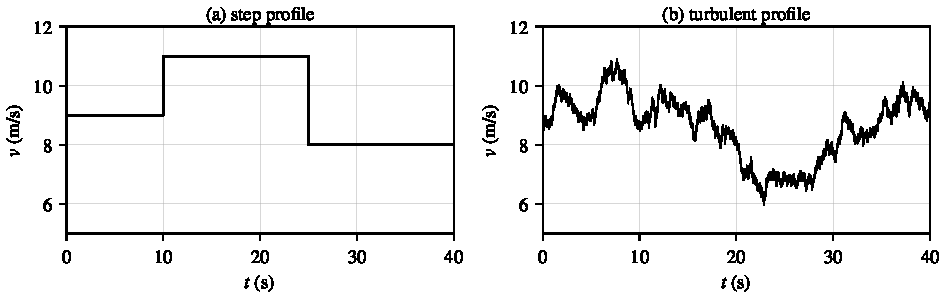
\includegraphics[width=\textwidth]{wind.pdf}
\caption{Wind profiles: (\textbf{a}) step wind; (\textbf{b}) random wind.}
\label{fig:wind}
\end{figure}

The speed tracking is evaluated from $t=1$~s by
\begin{equation}
\begin{gathered}
\mathrm{RMSE}=\sqrt{\frac1N\sum_{k=1}^Ne_\Omega^2(k)},\qquad
\mathrm{MAE}=\frac1N\sum_{k=1}^N|e_\Omega(k)|,\qquad
e_{\max}=\max_k|e_\Omega(k)|,\\
\mathrm{IAE}=\int|e_\Omega|\,dt,\qquad
\mathrm{ISE}=\int e_\Omega^2\,dt .
\end{gathered}
\label{eq:metrics}
\end{equation}

\subsection{Case 1: Step Wind}
Figure~\ref{fig:speed}a shows that the measured rotor speed follows the MPPT reference from 1.82 to 2.23
and then 1.62~rad/s. After each wind step, the speed error returns within 2~mrad/s in 1.9~s with the
network, instead of 3.9 to 4.4~s without it. Figure~\ref{fig:currents} shows that $i_{sq}$ and $i_{gd}$
follow their references during the transients, while $i_{sd}$ and $i_{gq}$ remain around zero with the
measurement noise and, for the grid current, the 300~Hz ripple due to the grid harmonics.
Figure~\ref{fig:torque}a shows that the electromagnetic torque follows its reference; the torque ripple
is 0.55\,\% of $T_n$ (standard deviation). The difference between $-T_e$ and $T_w$ accelerates or
decelerates the rotor towards the new optimal speed. Figure~\ref{fig:dclink}a shows that the DC-link
voltage stays within 7~V (0.6\,\%) of 1200~V during the steps, thanks to the feedforward of $P_{dc}$.

\begin{figure}[!htb]
\centering
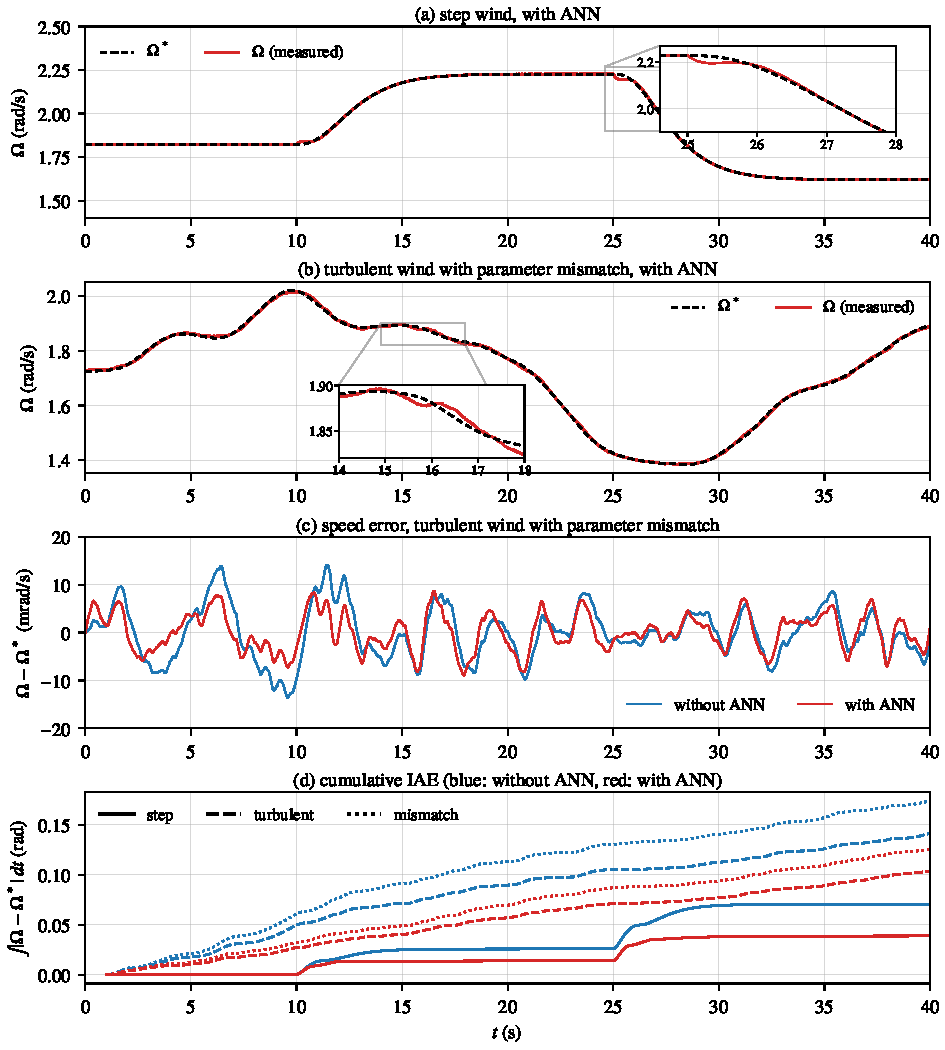
\includegraphics[width=\textwidth]{speed.pdf}
\caption{Rotor speed tracking: (\textbf{a}) step wind; (\textbf{b}) random wind with parameter
uncertainty; (\textbf{c}) speed error without and with the RBF network in case 3; (\textbf{d}) cumulative
IAE in cases 1 to 3.}
\label{fig:speed}
\end{figure}

\begin{figure}[!htb]
\centering
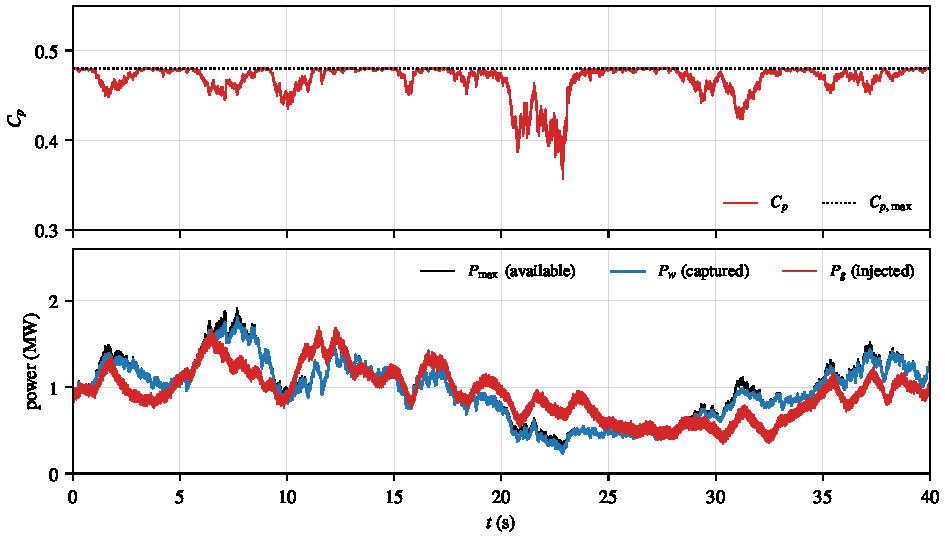
\includegraphics[width=\textwidth]{power_cp.pdf}
\caption{Random wind with nominal parameters: power coefficient (\textbf{top}) and maximum available,
captured and injected powers (\textbf{bottom}).}
\label{fig:power}
\end{figure}

\subsection{Case 2: Random Wind}
Figure~\ref{fig:power} shows the MPPT performance under random wind. The power coefficient stays close to
$C_{p,\max}$, except during the fast wind decrease around 22~s, where the inertia prevents the rotor from
slowing down quickly. The captured power follows the maximum available power, and the difference between
the captured and the injected powers corresponds to the kinetic energy stored in or released by the rotor.
The MPPT efficiency, i.e., the ratio between the captured energy and the maximum available energy, is
97.7\,\%. Figure~\ref{fig:thd} shows the grid current at 20~s: its THD is 3.9\,\%, mainly due to the 5th
(3.6\,\%) and 7th (1.6\,\%) harmonics imposed by the grid voltage, and every harmonic is below the limit
of IEEE Std 519~\cite{ieee519}.

\begin{figure}[!htb]
\centering
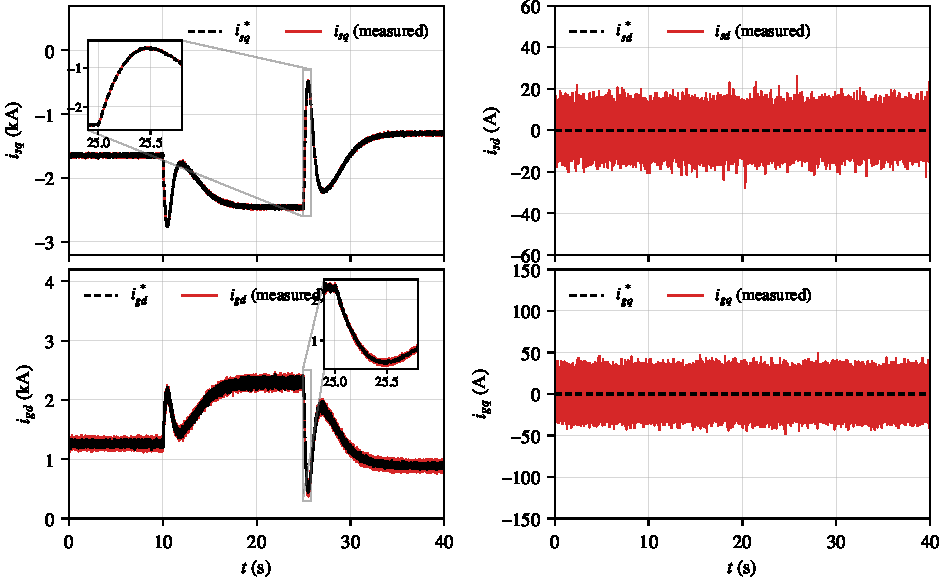
\includegraphics[width=\textwidth]{currents.pdf}
\caption{Step wind, control with the RBF network: references (dashed) and measured values (solid) of the
stator and grid currents.}
\label{fig:currents}
\end{figure}

\begin{figure}[!htb]
\centering
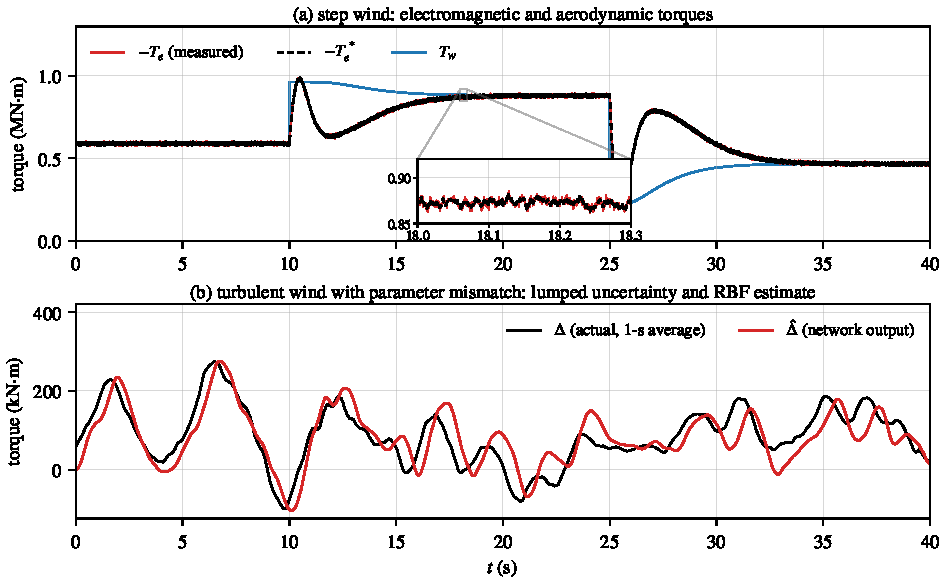
\includegraphics[width=\textwidth]{torque.pdf}
\caption{(\textbf{a}) Electromagnetic torque, its reference and aerodynamic torque under step wind, with
an enlarged view of the torque ripple; (\textbf{b}) lumped uncertainty $\Delta$ and its RBF estimate
$\hat\Delta$ in case 3.}
\label{fig:torque}
\end{figure}

\subsection{Case 3: Parameter Uncertainty}
With the parameter mismatch, the rotor speed still follows its reference (Figure~\ref{fig:speed}b). The
speed error is smaller with the network (Figure~\ref{fig:speed}c), and the cumulative IAE grows more
slowly in the three cases (Figure~\ref{fig:speed}d). Figure~\ref{fig:torque}b shows that the network output
follows the lumped uncertainty: their mean values are 82.5 and 83.4~kN$\cdot$m, i.e., about 14\,\% of the
aerodynamic torque. Figure~\ref{fig:pq}a shows that the injected active power follows the wind power and
that the reactive power remains around zero; the power factor is 1.00.

\begin{figure}[!htb]
\centering
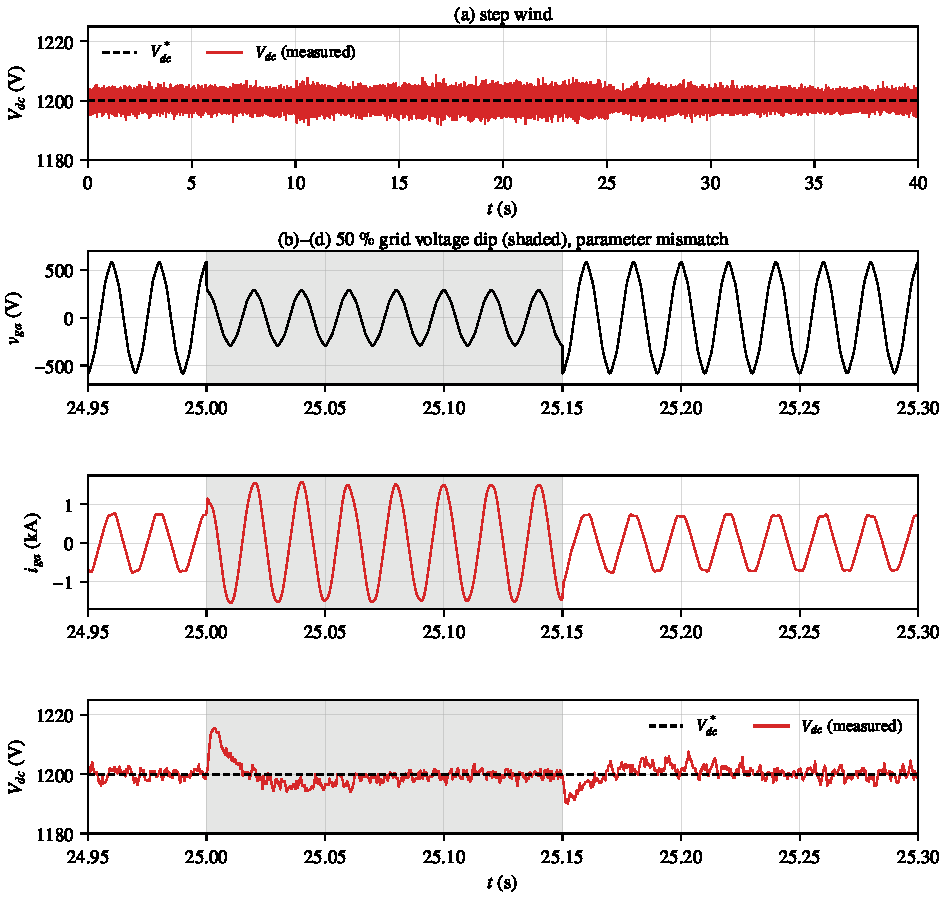
\includegraphics[width=\textwidth]{dclink.pdf}
\caption{DC-link voltage under step wind (\textbf{a}), and grid voltage (\textbf{b}), grid current
(\textbf{c}) and DC-link voltage (\textbf{d}) during the 50\,\% voltage dip of case 4.}
\label{fig:dclink}
\end{figure}

\begin{figure}[!htb]
\centering
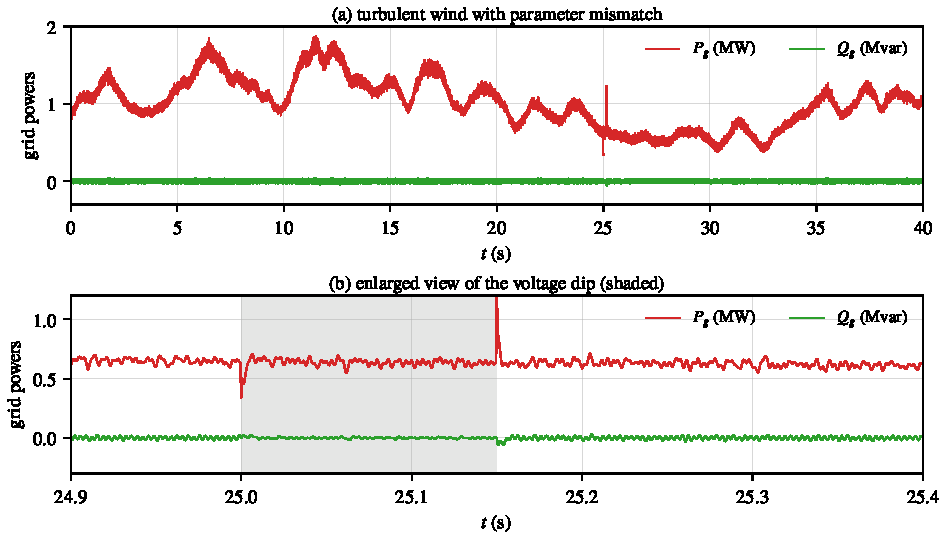
\includegraphics[width=\textwidth]{pq.pdf}
\caption{Active and reactive grid powers in cases 3 and 4: (\textbf{a}) whole simulation;
(\textbf{b}) enlarged view of the voltage dip.}
\label{fig:pq}
\end{figure}

\begin{figure}[!htb]
\centering
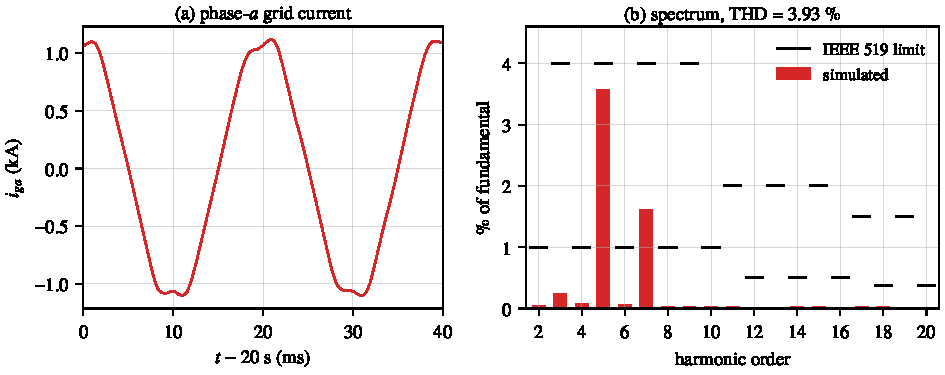
\includegraphics[width=\textwidth]{thd.pdf}
\caption{Random wind, $t=20$~s: (\textbf{a}) phase-$a$ grid current; (\textbf{b}) harmonic spectrum and
individual limits of IEEE Std 519.}
\label{fig:thd}
\end{figure}

\subsection{Case 4: Grid Voltage Dip}
During the 50\,\% voltage dip (Figure~\ref{fig:dclink}b--d), the grid current doubles, from 0.77 to
1.50~kA, to keep the injected power, which remains below the current limit of the converter. The DC-link
voltage deviates by 16~V (1.3\,\%) at the beginning of the dip and returns within 5~V of 1200~V about
50~ms after its end. The active power is maintained, with short transients at the beginning and at the
end of the dip, and the reactive power remains below 61~kvar (Figure~\ref{fig:pq}b).

\subsection{Quantitative Assessment}
Table~\ref{tab:speed} summarizes the speed tracking. With the network, the IAE decreases by 44.8\,\% in
case 1, 26.5\,\% in case 2 and 27.9\,\% in case 3, and the ISE decreases by 46 to 52\,\%, with the same
nominal gains. Table~\ref{tab:sys} shows that the other variables are practically unchanged: the current
errors, the DC-link deviation, the torque ripple and the grid-current THD are the same, and the captured
energy and the MPPT efficiency are equal. The network therefore improves the variable that it compensates,
the rotor speed, without degrading the rest of the system. Its price is a slightly more active torque, with
a 9 to 12\,\% larger standard deviation of the rate of the 50-ms averaged torque. The remaining speed error
comes mainly from the anemometer delay, which no model-based compensation can remove, and from the
measurement noise.

\begin{table}[!htb]
\caption{Speed tracking performance without and with the adaptive RBF compensation (best values in bold).}
\label{tab:speed}
\centering
\setlength{\tabcolsep}{5pt}
\begin{tabular}{llccc}
\toprule
Case & Metric & Without ANN & With ANN & Improvement (\%)\\
\midrule
1. Step wind & RMSE (mrad/s) & 4.99 & \textbf{3.67} & 26.5\\
 & MAE (mrad/s) & 1.81 & \textbf{1.00} & 44.8\\
 & $e_{\max}$ (mrad/s) & 33.2 & \textbf{30.1} & 9.5\\
 & IAE (mrad) & 70.6 & \textbf{39.0} & 44.8\\
 & ISE ($10^{-4}$ rad$^2$/s) & 9.71 & \textbf{5.24} & 46.0\\
 & settling to 2 mrad/s (s) & 3.85--4.35 & \textbf{1.88} & 51--57\\
\midrule
2. Random wind & RMSE (mrad/s) & 4.61 & \textbf{3.25} & 29.6\\
 & MAE (mrad/s) & 3.63 & \textbf{2.66} & 26.5\\
 & $e_{\max}$ (mrad/s) & 12.7 & \textbf{7.42} & 41.4\\
 & IAE (mrad) & 141.4 & \textbf{103.9} & 26.5\\
 & ISE ($10^{-4}$ rad$^2$/s) & 8.28 & \textbf{4.11} & 50.4\\
\midrule
3. Uncertainty & RMSE (mrad/s) & 5.55 & \textbf{3.87} & 30.4\\
 & MAE (mrad/s) & 4.47 & \textbf{3.22} & 27.9\\
 & $e_{\max}$ (mrad/s) & 14.2 & \textbf{8.93} & 37.0\\
 & IAE (mrad) & 174.3 & \textbf{125.7} & 27.9\\
 & ISE ($10^{-4}$ rad$^2$/s) & 12.0 & \textbf{5.83} & 51.5\\
\bottomrule
\end{tabular}
\end{table}

\begin{table}[!htb]
\caption{Performance of the whole system without and with the adaptive RBF compensation (40~s, from
$t=1$~s; best values in bold, both in bold when the difference is negligible).}
\label{tab:sys}
\centering
\footnotesize
\setlength{\tabcolsep}{4pt}
\begin{tabular}{lcccccc}
\toprule
 & \multicolumn{2}{c}{1. Step wind} & \multicolumn{2}{c}{2. Random wind} & \multicolumn{2}{c}{3--4. Uncertainty, dip}\\
\cmidrule(lr){2-3}\cmidrule(lr){4-5}\cmidrule(lr){6-7}
Metric & Without & With & Without & With & Without & With\\
\midrule
Max $|V_{dc}-V_{dc}^*|$ (V)$^{1}$ & \textbf{6.96} & \textbf{6.94} & \textbf{7.03} & \textbf{6.90} & \textbf{9.32} & \textbf{9.10}\\
Max $|V_{dc}-V_{dc}^*|$ in the dip (V) & -- & -- & -- & -- & \textbf{16.1} & \textbf{15.6}\\
RMS error of $i_{sq}$ (A) & \textbf{5.83} & \textbf{5.80} & \textbf{5.85} & \textbf{5.81} & \textbf{5.81} & \textbf{5.79}\\
RMS error of $i_{gd}$ (A) & \textbf{41.5} & \textbf{41.4} & \textbf{42.3} & \textbf{42.3} & \textbf{35.1} & \textbf{35.0}\\
Torque ripple (\% of $T_n$)$^{2}$ & \textbf{0.55} & \textbf{0.54} & \textbf{0.60} & \textbf{0.60} & \textbf{0.61} & \textbf{0.60}\\
Grid-current THD (\%) & \textbf{1.45} & \textbf{1.45} & \textbf{3.86} & \textbf{3.92} & \textbf{2.55} & \textbf{2.58}\\
Energy (kWh) & \textbf{13.86} & \textbf{13.86} & \textbf{10.05} & \textbf{10.04} & \textbf{10.98} & \textbf{10.97}\\
MPPT efficiency (\%) & \textbf{98.0} & \textbf{98.0} & \textbf{97.7} & \textbf{97.7} & \textbf{97.7} & \textbf{97.7}\\
Torque rate std (MN$\cdot$m/s)$^{3}$ & \textbf{0.239} & 0.267 & \textbf{0.212} & 0.231 & \textbf{0.210} & 0.233\\
\bottomrule
\end{tabular}

\vspace{2pt}{\footnotesize $^{1}$ outside the voltage dip; $^{2}$ standard deviation of $T_e$ minus its 50-ms average; $^{3}$ of the 50-ms averaged torque.}
\end{table}

%=====================================================================
\section{Conclusions}
This paper proposed a hybrid control for a 2~MW direct-drive PMSG wind energy conversion system in which
flatness generates the references, passivity-based control guarantees the energy structure and the
damping of the current loops of both converters, and an adaptive RBF network compensates the
aerodynamic-torque and parameter uncertainty. The system was modeled from the wind to the grid with an
exact energy balance, and a composite Lyapunov analysis showed that all closed-loop signals remain bounded,
that the current errors converge to zero and that the speed error converges to a neighborhood of zero
that depends on the approximation error of the network. Simulations with sensor noise and grid harmonics
under step wind, random wind, parameter uncertainty and a 50\,\% voltage dip showed that all the controlled
variables track their references, that the DC-link voltage remains within 0.8\,\% of its reference outside
the dip and within 1.3\,\% during it, that the grid-current THD stays below 4\,\%, and that the network
reduces the integral absolute speed error by 26.5 to 44.8\,\% with the same nominal gains and the same
captured energy.

The validation was made with the average model of the converters, so the switching ripple is not
represented, with an ideal synchronization to the grid and one realization of the random wind. No
experimental or hardware-in-the-loop (HIL) validation has yet been performed, and the stability analysis
does not include the sampling and the saturations. Future work will consider a switching model with an
$LCL$ filter, the dynamics of the phase-locked loop, HIL implementation, and comparisons with other
nonlinear controllers.

\vspace{10pt}
\noindent\small\textbf{Author Contributions:} Conceptualization, M.M. and K.K.; Methodology, S.R.;
Validation, S.R. and K.K.; Investigation, S.R.; Writing---original draft, S.R., M.M. and K.K.;
Supervision, M.M. and K.K.; Project administration, M.M. and K.K. All authors have read and agreed to the
published version of the manuscript.

\noindent\textbf{Funding:} This research received no external funding.

\noindent\textbf{Data Availability Statement:} The original contributions presented in this study are
included in the article. Further inquiries can be directed to the corresponding author.

\noindent\textbf{Conflicts of Interest:} The authors declare no conflicts of interest.
\normalsize

\begin{thebibliography}{99}
\small
\bibitem{barthelmie2021} Barthelmie, R.J.; Pryor, S.C. Climate Change Mitigation Potential of Wind Energy.
\emph{Climate} \textbf{2021}, \emph{9}, 136. https://doi.org/10.3390/cli9090136.
\bibitem{iea2024} International Energy Agency (IEA). \emph{World Energy Outlook 2024}; IEA: Paris, France, 2024.
\bibitem{gwec2024} Global Wind Energy Council (GWEC). \emph{Global Wind Report 2024}; GWEC: Brussels,
Belgium, 2024.
\bibitem{polinder2013} Polinder, H.; Ferreira, J.A.; Jensen, B.B.; Abrahamsen, A.B.; Atallah, K.;
McMahon, R.A. Trends in Wind Turbine Generator Systems. \emph{IEEE J. Emerg. Sel. Top. Power Electron.}
\textbf{2013}, \emph{1}, 174--185.
\bibitem{yaramasu2015} Yaramasu, V.; Wu, B.; Sen, P.C.; Kouro, S.; Narimani, M. High-Power Wind Energy
Conversion Systems: State-of-the-Art and Emerging Technologies. \emph{Proc. IEEE} \textbf{2015},
\emph{103}, 740--788.
\bibitem{wu2011} Wu, B.; Lang, Y.; Zargari, N.; Kouro, S. \emph{Power Conversion and Control of Wind
Energy Systems}; Wiley-IEEE Press: Hoboken, NJ, USA, 2011.
\bibitem{rolan2009} Rol\'an, A.; Luna, A.; V\'azquez, G.; Aguilar, D.; Azevedo, G. Modeling of a
Variable Speed Wind Turbine with a Permanent Magnet Synchronous Generator. In Proceedings of the IEEE
International Symposium on Industrial Electronics (ISIE), Seoul, Republic of Korea, 2009; pp.~734--739.
https://doi.org/10.1109/ISIE.2009.5218120.
\bibitem{aimene2022} Aimene, M.; Payman, A.; Dakyo, B. Comparative Study between Flatness-Based and
Field-Oriented Control Methods of a Grid-Connected Wind Energy Conversion System. \emph{Processes}
\textbf{2022}, \emph{10}, 378. https://doi.org/10.3390/pr10020378.
\bibitem{chinchilla2006} Chinchilla, M.; Arnaltes, S.; Burgos, J.C. Control of Permanent-Magnet
Generators Applied to Variable-Speed Wind-Energy Systems Connected to the Grid. \emph{IEEE Trans. Energy
Convers.} \textbf{2006}, \emph{21}, 130--135.
\bibitem{yazdani2010} Yazdani, A.; Iravani, R. \emph{Voltage-Sourced Converters in Power Systems:
Modeling, Control, and Applications}; Wiley-IEEE Press: Hoboken, NJ, USA, 2010.
\bibitem{blaabjerg2006} Blaabjerg, F.; Teodorescu, R.; Liserre, M.; Timbus, A.V. Overview of Control and
Grid Synchronization for Distributed Power Generation Systems. \emph{IEEE Trans. Ind. Electron.}
\textbf{2006}, \emph{53}, 1398--1409.
\bibitem{mechter2015} Mechter, A.; Kemih, K.; Ghanes, M. Sliding Mode Control of a Wind Turbine with
Exponential Reaching Law. \emph{Acta Polytech. Hung.} \textbf{2015}, \emph{12}, 167--183.
\bibitem{benabdeeseelam2025} Benabdeeseelam, A.; Messadi, M.; Kemih, K.; Hamiche, H. Chattering-Free
Terminal Sliding Mode Control Based on Adaptive Exponential Reaching Barrier Function for a Chaotic
Permanent Magnet Synchronous Generator in Offshore Wind Turbine System. \emph{Chin. Phys. B}
\textbf{2025}, \emph{34}, 090501.
\bibitem{mechter2016} Mechter, A.; Kemih, K.; Ghanes, M. Backstepping Control of a Wind Turbine for Low
Wind Speeds. \emph{Nonlinear Dyn.} \textbf{2016}, \emph{84}, 2435--2445.
https://doi.org/10.1007/s11071-016-2655-y.
\bibitem{messadi2015} Messadi, M.; Mellit, A.; Kemih, K.; Ghanes, M. Predictive Control of a Chaotic
Permanent Magnet Synchronous Generator in a Wind Turbine System. \emph{Chin. Phys. B} \textbf{2015},
\emph{24}, 010502.
\bibitem{yang2021} Yang, L.; Yang, F.; Sheng, W.; Zhou, K.; Huang, T. Fuzzy Chaos Control of Fractional
Order D-PMSG for Wind Turbine with Uncertain Parameters by State Feedback Design. \emph{Energies}
\textbf{2021}, \emph{14}, 7369.
\bibitem{fliess1995} Fliess, M.; L\'evine, J.; Martin, P.; Rouchon, P. Flatness and Defect of Non-Linear
Systems: Introductory Theory and Examples. \emph{Int. J. Control} \textbf{1995}, \emph{61}, 1327--1361.
\bibitem{thounthong2010} Thounthong, P.; Pierfederici, S.; Davat, B. Analysis of Differential
Flatness-Based Control for a Fuel Cell Hybrid Power Source. \emph{IEEE Trans. Energy Convers.}
\textbf{2010}, \emph{25}, 909--920.
\bibitem{ortega1998} Ortega, R.; Lor\'ia, A.; Nicklasson, P.J.; Sira-Ram\'irez, H.
\emph{Passivity-Based Control of Euler-Lagrange Systems}; Springer: London, UK, 1998.
\bibitem{ortega2002} Ortega, R.; van der Schaft, A.; Maschke, B.; Escobar, G. Interconnection and
Damping Assignment Passivity-Based Control of Port-Controlled Hamiltonian Systems. \emph{Automatica}
\textbf{2002}, \emph{38}, 585--596.
\bibitem{park1991} Park, J.; Sandberg, I.W. Universal Approximation Using Radial-Basis-Function
Networks. \emph{Neural Comput.} \textbf{1991}, \emph{3}, 246--257.
\bibitem{lewis1999} Lewis, F.L.; Jagannathan, S.; Ye\c{s}ildirek, A. \emph{Neural Network Control of
Robot Manipulators and Nonlinear Systems}; Taylor \& Francis: London, UK, 1999.
\bibitem{ioannou1996} Ioannou, P.A.; Sun, J. \emph{Robust Adaptive Control}; Prentice Hall: Upper Saddle
River, NJ, USA, 1996.
\bibitem{li2024} Li, Y.; Sun, W.; Yu, D. RBFNN-Based Global Fast Terminal Sliding Mode Control for Fully
Controlled Doubly Fed Induction Generator. \emph{J. Frankl. Inst.} \textbf{2024}, \emph{361}, 107196.
https://doi.org/10.1016/j.jfranklin.2024.107196.
\bibitem{bounar2025} Bounar, N.; Boulkroune, A.; Labdai, S.; Chrifi-Alaoui, L.; Khebbache, H.
Disturbance Observer-Based Finite-Time Adaptive Neural Control Scheme of DFIG-Wind Turbine. \emph{Wind
Eng.} \textbf{2025}, \emph{49}, 271--289. https://doi.org/10.1177/0309524X241263517.
\bibitem{dardabi2024} Dardabi, C.; Djebli, A.; Chojaa, H. Enhancing the Control of Doubly Fed Induction
Generators Using Artificial Neural Networks in the Presence of Real Wind Profiles. \emph{PLoS ONE}
\textbf{2024}, \emph{19}, e0300527. https://doi.org/10.1371/journal.pone.0300527.
\bibitem{regani2026} Regani, S.; Messadi, M.; Kemih, K. A Novel Chaos Control Approach with Adaptive ANN
Compensation for a DFIG-Based Wind Turbine. \emph{Mathematics} \textbf{2026}, \emph{14}, 3739.
https://doi.org/10.3390/math14203739.
\bibitem{hasan2021} Hasan, S.M.M.; Shatil, A.H.M. Design and Comparison of Grid Connected Permanent
Magnet Synchronous Generator Non-Salient Pole and Salient Pole Rotor Wind Turbine. \emph{AIUB J. Sci.
Eng.} \textbf{2021}, \emph{20}, 40--46.
\bibitem{heier2014} Heier, S. \emph{Grid Integration of Wind Energy: Onshore and Offshore Conversion
Systems}, 3rd ed.; Wiley: Chichester, UK, 2014.
\bibitem{khalil2002} Khalil, H.K. \emph{Nonlinear Systems}, 3rd ed.; Prentice Hall: Upper Saddle River,
NJ, USA, 2002.
\bibitem{ieee519} \emph{IEEE Std 519-2014}; IEEE Recommended Practice and Requirements for Harmonic
Control in Electric Power Systems. IEEE: New York, NY, USA, 2014.
\end{thebibliography}

\end{document}
